\section{第一周数值分析实验}
\subsection{第一节:级数求和与二元函数绘图}
\begin{ex}
编程求$\sum_{n=1}^{12}{n!}$的值.
\end{ex}
\lstinputlisting[language=matlab]{day1/work1q1.m}
\qa 522956313
\begin{ex}
绘制二元函数图像.
$$
f(x,y)=x^4-2x^2y+x^2-2xy+2y^2+\frac{9}{2}x-4y+4\,\,\,\,\left( -2\le x\le 3,-1\le y\le 7 \right) 
$$
\end{ex}
\lstinputlisting[language=matlab]{day1/work1q2.m}
\qa 
\begin{figure}[H]
	\centering
	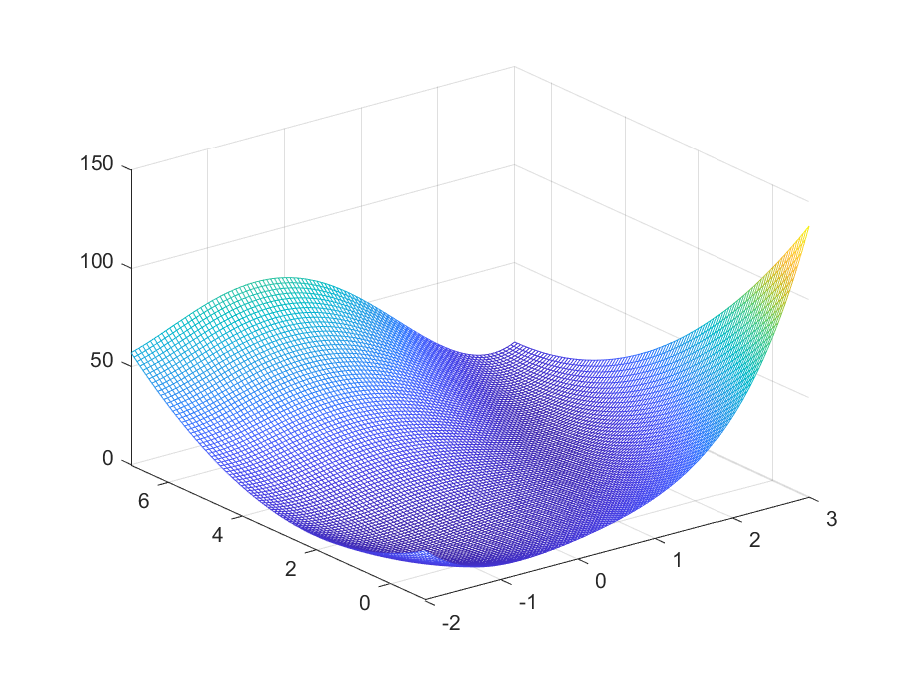
\includegraphics[width = 0.6\linewidth]{day1/q2.eps}
	\caption{运行结果}
\end{figure}
\subsection{第二节:积分递推公式}
\begin{ex}
	计算$I_n=e^{-1}\int_0^1{x^ne^xdx},(n=0,1,2,\cdots)$并估计误差
	
	方法1:利用递推公式 (A)
	$$
	\left( A \right) \text{ }\left\{ \begin{array}{l}
		I_n=1-nI_{n-1},\text{ }n=1,2,\cdots ,20\\
		I_0=1-e^{-1}\approx 0.6321.\\
	\end{array} \right. 
	$$
	
	方法2:利用递推公式 (B)
	$$
	\left( B \right) \left\{ \begin{array}{l}
		\widetilde{I_{20}}=?;\\
		\widetilde{I}_{n-1}=\frac{1}{n}\left( 1-\widetilde{I_n} \right) ,\text{ \,\,}n=19,\cdots ,9,8,\cdots 0.\\
	\end{array} \right. 
	$$
\end{ex}
\lstinputlisting[language=matlab]{day1/work1q3.m}
\qa 
% Table generated by Excel2LaTeX from sheet 'Sheet1'
\begin{table}[H]
	\centering
	\caption{运行结果}
	\resizebox{1\columnwidth}{!}{
	\begin{tabular}{c|cccccccccc}
		n     & 1     & 2     & 3     & 4     & 5     & 6     & 7     & 8     & 9     & 10 \\
		IA    & 0.3679 & 0.2642 & 0.2074 & 0.1704 & 0.148 & 0.112 & 0.216 & -0.728 & 7.552 & -74.52 \\
		EA    & 5.00E-05 & 5.00E-05 & 0.0001 & 0.0003 & 0.0012 & 0.006 & 0.036 & 0.252 & 2.016 & 18.144 \\
		n     & 11    & 12    & 13    & 14    & 15    & 16    & 17    & 18    & 19    & 20 \\
		IA    & 820.72 & -9847.64 & 128020.3 & -1792283 & 26884253 & -4.3E+08 & 7.31E+09 & -1.3E+11 & 2.5E+12 & -5E+13 \\
		EA    & 181.44 & 1995.84 & 23950.08 & 311351 & 4358915 & 65383718 & 1.05E+09 & 1.78E+10 & 3.2E+11 & 6.08E+12 \\
		\hline
		n     & 1     & 2     & 3     & 4     & 5     & 6     & 7     & 8     & 9     & 10 \\
		IB    & 0.367879 & 0.264241 & 0.207277 & 0.170893 & 0.145533 & 0.126802 & 0.112384 & 0.100932 & 0.091612 & 0.083877 \\
		EB    & 2.06E-20 & 4.11E-20 & 1.23E-19 & 4.93E-19 & 2.47E-18 & 1.48E-17 & 1.04E-16 & 8.29E-16 & 7.46E-15 & 7.46E-14 \\
		n     & 11    & 12    & 13    & 14    & 15    & 16    & 17    & 18    & 19    & 20 \\
		IB    & 0.077352 & 0.071773 & 0.066948 & 0.062732 & 0.059018 & 0.05572 & 0.052768 & 0.05018 & 0.04658 & 0.0684 \\
		EB    & 8.20E-13 & 9.84E-12 & 1.28E-10 & 1.79E-09 & 2.69E-08 & 4.30E-07 & 7.31E-06 & 0.000132 & 0.0025 & 0.05 \\
	\end{tabular}%
	}
	\label{tab:addlabel1}%
\end{table}%
\begin{ex}
	计算$I_n=\int_0^1{\frac{x^n}{x+5}dx},(n=0,1,2,\cdots 20)$并估计误差.
\end{ex}
\lstinputlisting[language=matlab]{day1/work1q4.m}
\qa 
% Table generated by Excel2LaTeX from sheet 'Sheet1'
\begin{table}[H]
	\centering
	\caption{运行结果}
	\resizebox{1\columnwidth}{!}{
	\begin{tabular}{c|cccccccccc}
		n     & 1     & 2     & 3     & 4     & 5     & 6     & 7     & 8     & 9     & 10 \\
		IA    & 0.0885 & 0.0575 & 0.045833 & 0.020833 & 0.095833 & -0.3125 & 1.705357 & -8.40179 & 42.12004 & -210.5 \\
		EA    & 5.00E-06 & 2.50E-05 & 0.000125 & 0.000625 & 0.003125 & 0.015625 & 0.078125 & 0.390625 & 1.953125 & 9.765625 \\
		n     & 11    & 12    & 13    & 14    & 15    & 16    & 17    & 18    & 19    & 20 \\
		IA    & 1052.592 & -5262.88 & 26314.46 & -131572 & 657861.2 & -3289306 & 16446529 & -8.2E+07 & 4.11E+08 & -2.1E+09 \\
		EA    & 48.82813 & 244.1406 & 1220.703 & 6103.516 & 30517.58 & 152587.9 & 762939.5 & 3814697 & 19073486 & 95367432 \\
		\hline
		n     & 1     & 2     & 3     & 4     & 5     & 6     & 7     & 8     & 9     & 10 \\
		IB    & 0.088392 & 0.058039 & 0.043139 & 0.034306 & 0.028468 & 0.024325 & 0.021233 & 0.018837 & 0.016926 & 0.015368 \\
		EB    & 2.62E-18 & 1.31E-17 & 6.55E-17 & 3.28E-16 & 1.64E-15 & 8.19E-15 & 4.10E-14 & 2.05E-13 & 1.02E-12 & 5.12E-12 \\
		n     & 11    & 12    & 13    & 14    & 15    & 16    & 17    & 18    & 19    & 20 \\
		IB    & 0.014071 & 0.012977 & 0.01204 & 0.011229 & 0.010521 & 0.009896 & 0.009342 & 0.008846 & 0.008402 & 0.00799 \\
		EB    & 2.56E-11 & 1.28E-10 & 6.40E-10 & 3.20E-09 & 1.60E-08 & 8.00E-08 & 4.00E-07 & 2.00E-06 & 1.00E-05 & 5.00E-05 \\
	\end{tabular}%
	}
	\label{tab:addlabel2}%
\end{table}%
